\documentclass{standalone}
\usepackage{tikz} 
\usetikzlibrary{calc}
\usetikzlibrary{arrows.meta}
\usepackage{siunitx} 
\usepackage{charter}
\usepackage{parskip}

\begin{document}        
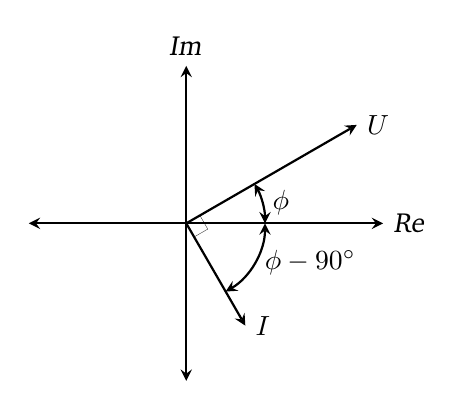
\begin{tikzpicture}[>=stealth]
%\begin{tikzpicture}[]
\draw[style=help lines] (0,0) (3,2);

\coordinate (vec1) at (300:1.5); 
\coordinate (vec2) at (30:2.5);
\coordinate (vec3) at (0:2.5);
\coordinate (vec4) at (90:2);
\coordinate (vec5) at (270:2);
\coordinate (vec6) at (180:2);
\coordinate (vec7) at (300:0.3);
\coordinate (vec8) at (30:0.3);

\draw[->,thick,black] (0,0) -- (vec1) node[right] {$I$};
\draw[->,thick,black] (0,0) -- (vec2) node[right] {$U$};
\draw[->,thick,black] (0,0) -- (vec3) node [right] {\textsl{Re}};
\draw[->,thick,black] (0,0) -- (vec4) node [above] {\textsl{Im}};
\draw[->,thick,black] (0,0) -- (vec5);
\draw[->,thick,black] (0,0) -- (vec6);

\draw [<->, thick] (1.0,0) arc [start angle=0, end angle=30, radius=1cm]
    node [midway, right] {$\phi$};    

\draw [<->, thick] (1.0,0) arc [start angle=0, end angle=-60, radius=1cm]
    node [midway, right] {$\phi-\ang{90}$};
    
\draw [ultra thin, rotate=30] (0,-0.2) -- (0.2,-0.2) -- (0.2,0);
\end{tikzpicture}

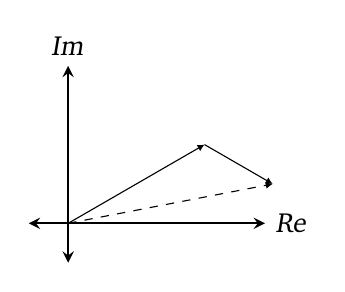
\begin{tikzpicture}[>=stealth]
\draw[style=help lines] (0,0) (3,2);
\coordinate (vec1) at (330:1); 
\coordinate (vec2) at (30:2);
\coordinate (vec21) at (30:1.969);
\coordinate (vec3) at (0:2.5);
\coordinate (vec4) at (90:2);
\coordinate (vec5) at (270:0.5);
\coordinate (vec6) at (180:0.5);
\coordinate (vec7) at ($(vec1) + (vec2)$);
\draw[->,thick,black] (0,0) -- (vec3) node [right] {\textsl{Re}};
\draw[->,thick,black] (0,0) -- (vec4) node [above] {\textsl{Im}};
\draw[->,thick,black] (0,0) -- (vec5);
\draw[->,thick,black] (0,0) -- (vec6);

\draw[-{Latex[length=2.5pt,width=2.55pt]},,black] (0,0) -- (vec2);
\draw[-{Latex[length=2.5pt,width=2.55pt]},,black] (vec2)-- ++(vec1);
\draw[-{Latex[length=2.5pt,width=2.55pt]},,black,dashed] (0,0) -- (vec7);

\end{tikzpicture}

\end{document}